show gitig\documentclass[../main.tex]{subfiles}
% 2.2.1 Was ist es?
Das klassische Doppelspaltexperiment weist das Wellenartige Verhalten von Licht durch die Interferenz der Wellen nach.
% 2.2.2 Geschichte / Entdeckung
Das Experiment wurde erstmals 1801 von Thomas Young durchgeführt \cite{TODO}.

\begin{figure}[ht]
    \centering
    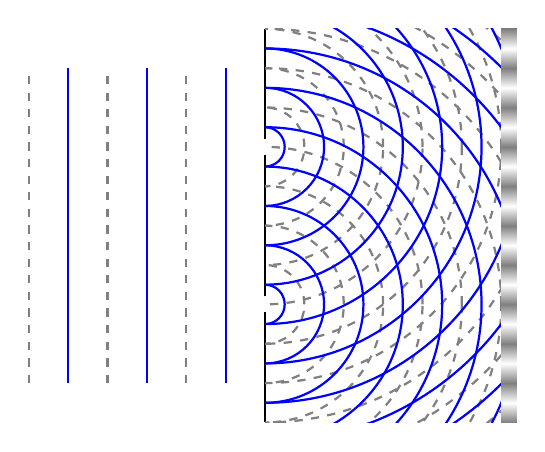
\begin{tikzpicture}
        %\draw[step=1] (0.5,1.5) grid (6.2,6.5);
        
        % Parallel Waves
        \foreach \i in {0.5,1.5,...,2.5}
            \draw[blue,thick] ({\i},2) -- ({\i},6); % Hochpunkte

        \foreach \i in {0,1,...,2.5}
            \draw[gray,dashed,thick] ({\i},2) -- ({\i},6); % Tiefpunkte
        
        % Double Slit @ 3 & 5
        \draw[thick] (3,1.5) -- (3,2.9);
        \draw[thick] (3,3.1) -- (3,4.9);
        \draw[thick] (3,5.1) -- (3,6.5);
        
        % Elementary waves
        \begin{scope}
            \clip (3,1.5) rectangle (6,6.5);
            
            \foreach \i in {0.5,1,...,5} { % Tiefpunkte
                \draw[gray, dashed,thick] (3,5) circle(\i);
                \draw[gray, dashed,thick] (3,3) circle(\i);
            }
            \foreach \i in {0.25,0.75,...,5} { % Hochpunkte
                \draw[blue,thick] (3,5) circle(\i);
                \draw[blue,thick] (3,3) circle(\i);
            }
        \end{scope}

        % Interference pattern
        \foreach \i in {1,2,...,20}
            \shade[black,white,shading angle={mod(\i,20)*180}] (6,{\i/4+1.25}) rectangle (6.2,{\i/4+1.5});
    \end{tikzpicture}
    \caption{Doppelspaltexperiment: Wellenhochpunkte blau, Wellentiefpunkte grau}
    \label{fig:doppelspalt}
\end{figure}
% 2.2.3 Aufbau
Der Aufbau ist wie folgt (Abb. \ref{fig:doppelspalt}): Links kommen Parallelwellen auf eine Wand mit zwei Spalten zu. Rechts daneben ist eine geschlossene Wand, auf der das Licht aufkommt.

% 2.2.4 Beobachtung
Die Lichtwellen werden am Doppelspalt in zwei Elementarwellen zerlegt. Diese überlappen und interferieren miteinander. Verfolgt man die Punkte konstruktiver Interferenz (Wellenhochpunkte, blau), gelangt man an die Maxima (Muster rechts, dunkel). Verfolgt man dagegen die Punkte destruktiver Interferenz (Wellentiefpunkte, grau), gelangt man an die Minima (Muster rechts, hell).
% 2.2.5 Schlussfolgerung
Die Maxima treten da auf, wo zwei Elementarwellen einen Gangunterschied eines Vielfachen von $\lambda$ haben, weil Konstruktive Interferenz auftritt (Gl. \ref{eq:konstruktive_interferenz}). Die Minima treten da auf, wo der Gangunterschied um $\frac{\lambda}{2}$ verschoben ist (Gl. \ref{eq:destruktive_interferenz}).


% 2.2._ Warum Grundlage?
% TODO